\documentclass{beamer}

\mode<presentation>
{
\usetheme{Frankfurt}
\setbeamercovered{transparent}
}

\title{Predicting Wine Quality: A Conundrum}
\subtitle{Would you like some cheese with that?}
\author{Kalbi Zongo, Song Hoa Choi, Gina Shellhammer, Matt Edwards}
\date{June 2, 2014}

\begin{document}
\begin{frame}
\titlepage
\end{frame}

\begin{frame}
\frametitle{Outline}
\tableofcontents
\end{frame}

% -------------------------------- INTRODUCTION --------------------------------------------------
\section{Introduction}
\begin{frame}{Task}
\textbf{Predict} the blind taster quality score of a wine based on chemical tests.

\end{frame}

\begin{frame}{Data}
\begin{itemize}
	\item Two Datasets: Red \& White vinho verde wine samples from northern Portugal
	\item[]
	\item 1599 \& 4898 rows, respectively
	\item[]
	\item 11 Explanatory variables: measurements from various phytochemicals in wine
	\item[]
	\item Response variable "quality" is discrete variable on ordered scale from 0 (worst) to 10 (best)
\end{itemize}
\end{frame}

\begin{frame}{Quality}
\begin{figure}
	\centering
	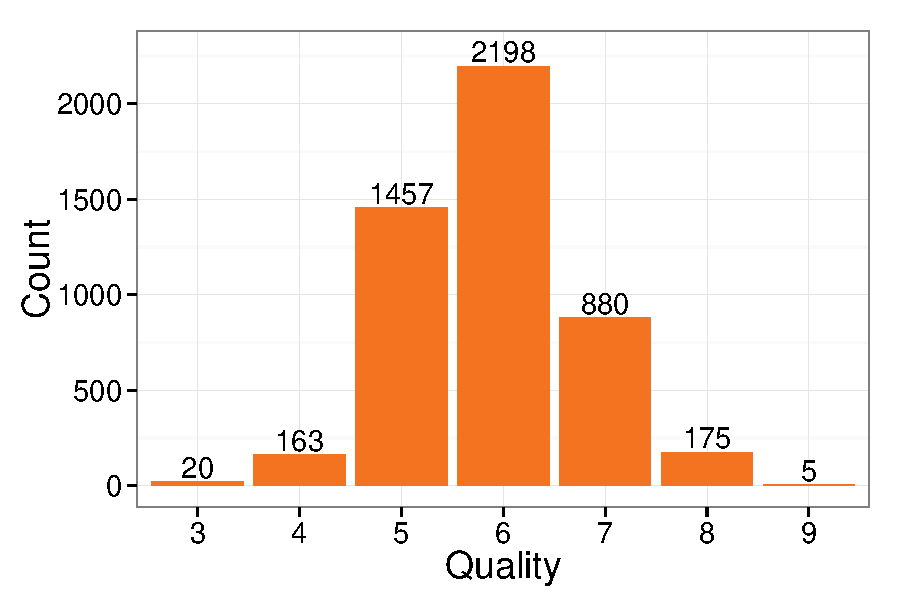
\includegraphics[width=\textwidth]{../images/white_hist.pdf}
\end{figure}
\end{frame}

% -------------------------------- MACHINE LEARNING METHODS --------------------------------------------------
\section{Machine Learning Methods}
\begin{frame}{Training and Testing Sets}
	\begin{itemize}
	\item Training and Testing set constructed through stratified sampling.
	\item[]
	\item Quality variable was the strata
	\item[]
	\item Why: Ensure representation of all quality categories in both Training \& Testing datasets.
	\item[]
	\item How: 37.5\% of items (rounded up) in strata were randomly selected to be in the testing set. Remaining 62.5\% were the training set.
	\item[]
	\item Same training \& testing sets used for each analysis type.
	\end{itemize}
\end{frame}


\begin{frame}{Regression}
content...
\end{frame}

\begin{frame}{Classification}
content...
\end{frame}

\begin{frame}{Random Randomness is Random}
	\begin{itemize}
	\item 75\% of Quality ratings were either 5 or 6. 
	\item[]
	\item Is randomly assigning 5 or 6 to everything as good as, or better than, our other methods?
	\item[]
	\item Using \texttt{rbinom(1,1,0.6014)}, 1s were predicted as quality 6, 0s as quality 5
	\item[]
	\item Probability of 60.14\% because from Training Set, considering only 5s and 6s, 6s were 60.14\% of total observations
	\item[]
	\item Our base line success rate to compare other methods.
	\end{itemize}
\end{frame}


% -------------------------------- FINDINGS --------------------------------------------------
\section{Findings}

\begin{frame}{Regression: 50\% Success Rate}
content... change success rate in title
\end{frame}

\begin{frame}{Classification: 50\% Success Rate}
content... change success rate in title
\end{frame}


\begin{frame}{Random 'Prediction': 39.67\% Success Rate}
	Turns out, that's not really a great 'prediction' method. Who knew?
	\begin{figure}
		\centering
		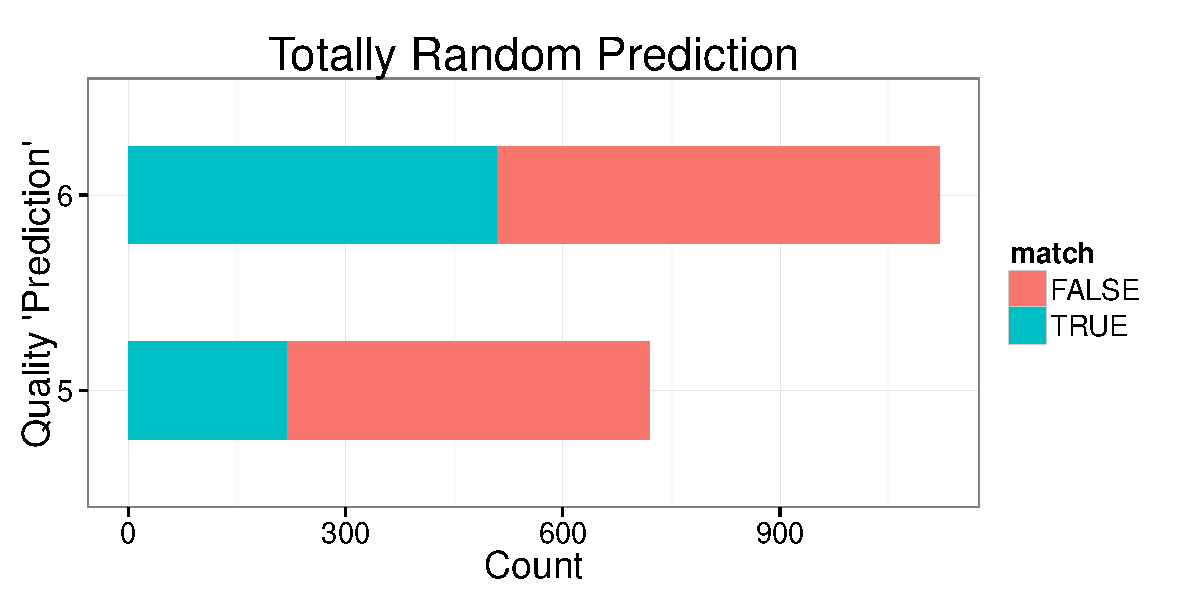
\includegraphics[width=\textwidth]{../images/RandomPrediction.pdf}
	\end{figure}
\end{frame}


% -------------------------------- DISCUSSION --------------------------------------------------
\section{Discussion}
\begin{frame}{}
content...

\end{frame}
\end{document}
